\documentclass[a4paper]{report}
\usepackage{setspace}
%\usepackage{subfigure}

\pagestyle{plain}
\usepackage{amssymb,graphicx,color}
\usepackage{amsfonts}
\usepackage{latexsym}
\usepackage{amsmath}
\usepackage[a4paper, margin = 3cm, bottom = 2.5cm]{geometry}

\newtheorem{theorem}{THEOREM}
\newtheorem{lemma}[theorem]{LEMMA}
\newtheorem{corollary}[theorem]{COROLLARY}
\newtheorem{proposition}[theorem]{PROPOSITION}
\newtheorem{remark}[theorem]{REMARK}
\newtheorem{definition}[theorem]{DEFINITION}
\newtheorem{fact}[theorem]{FACT}

\newtheorem{problem}[theorem]{PROBLEM}
\newtheorem{exercise}[theorem]{EXERCISE}
\def \set#1{\{#1\} }

\newenvironment{proof}{
PROOF:
\begin{quotation}}{
$\Box$ \end{quotation}}



\newcommand{\nats}{\mbox{\( \mathbb N \)}}
\newcommand{\rat}{\mbox{\(\mathbb Q\)}}
\newcommand{\rats}{\mbox{\(\mathbb Q\)}}
\newcommand{\reals}{\mbox{\(\mathbb R\)}}
\newcommand{\ints}{\mbox{\(\mathbb Z\)}}

%%%%%%%%%%%%%%%%%%%%%%%%%%


\title{{\vspace{-14em} 
\includegraphics[scale=0.4]{images/ucl_logo.png}}\\
{{\Huge Investigating the use of Reinforcement Learning Algorithms in Traffic Environments}}\\
% {\large Optional Subtitle}\\
}
\date{Submission date: Day Month Year}
\author{Abdul Muhaymin Abdul Hafiz\thanks{
{\bf Disclaimer:}
This report is submitted as part requirement for the BSc Degree in Computer Science at UCL. It is
substantially the result of my own work except where explicitly indicated in the text.
The report may be freely copied and distributed provided the source is explicitly acknowledged.
\newline  %% \\ messes it up
}
\\ \\
BSc Computer Science\\ \\
Supervisor: Prof. Graham Roberts}



\begin{document}
 
\onehalfspacing
\maketitle
\begin{abstract}
Summarise your report concisely.
\end{abstract}
\tableofcontents
\setcounter{page}{1}


\chapter{Introduction}

\section{The Problem}
Traffic lights are ubiquitous signalling devices used to control the flow of vehicle and pedestrian traffic, primarily for safety and better regulation of traffic. First introduced in 1868 on Parliament Square in London \cite{ThamesLeisureFacts2017}, there have been a wide range of designs created with the most common being a three-colour design -- that is green, amber, and red.

The three-colour de jure standard typically uses an internal clock to cycle through and control the duration of each signal phase in a pre-programmed pattern. Whilst this is an obvious approach, the fixed timer takes for granted that traffic demand will remain relatively constant over time, disregarding finer granularity and variations in conditions.

In an endeavour to improve upon this, advanced traffic light systems equipped with sensors are progressively being introduced. These systems dynamically adapt signal timings in response to observed traffic conditions by using rule-based logic and manually designed heuristics. This approach offers improvements in waiting times and vehicle throughput \cite{FHWA_ASCT17}, however it relies on predefined rules defined by domain experts that may fail to generalise and perform optimally in all conditions.

\section{Aims and Objectives}

The overall aim of this dissertation will be to perform a detailed analysis and evaluation of how an intelligent agent may be used to hopefully improve upon existing traffic light systems. Rather than explicitly defining behaviour in different traffic scenarios as before, we will observe how optimal decision-making policies may be learnt independently through the use of reinforcement learning algorithms.

Our first objective will be to define an environment in which our simulations and experiments will be conducted. Following this we will review the traffic light systems currently in use and then build an abstracted computer representation of the area. The next objective will then be to develop our intelligent agents progressively, going through various reinforcement learning algorithms to see what improvements are made. At each stage, the impact on both pedestrians and vehicles will be considered. We will also consider the impact of changing the road design in itself as a means of making improvements. Our final objective will then be to assess the feasibility of our agents and what factors would need to be considered in a tangible implementation.

Time is a currency that once spent cannot be regained. Traffic lights govern our lives to the extent that saving mere fractions of a second at the individual level can compound to an indescribable amount saved when considering the aggregate. By leveraging intelligent agents, this research hopes to take traffic lights a step further -- regardless of how big that step may be.

\section{Report Overview}
We will begin with defining the environment in which we will be conducting our traffic experiments, and then building out this environment using available open source tools and libraries. Whilst accuracy and scope of the environment are important, they will not take precedence over the implementation and analysis of the intelligent agents themselves.

Following this, the context and theory behind reinforcement learning itself will be explored, as well as definitions and terminology that will be used throughout the dissertation. These foundations will be necessary when explaining the motivation behind decisions made later on.

Next we will discuss the creation of an application programming interface that will enable us to connect to our environment for the purposes of observation and control. Based on the default environment and traffic light systems, we will also define a reward which will be used to evaluate performance.

Upon making our environment, we will implement and explore different reinforcement learning algorithms our intelligent agent may use -- namely Q-learning and Deep Q-learning. These discussions will be supplemented with the theory regarding how each works, as well as the improvements and limitations proposed by each. Further derivatives of these algorithms and the advantages they bring will also be briefly touched upon, however they will not be implemented.

Continuing from this, a novel approach in which multiple intelligent agents interface together through the use of a network layer will be detailed and implemented. The limitations imposed by such an approach will be considered, as well as how it may be implemented in practice outside of the simulated environment setting.

Finally, after testing and evaluating the different approaches in unforeseen traffic scenarios, we will draw our overall conclusions. Feasibility of such a project will be discussed, as well as interesting technical challenges that were encountered. Future work and limitations to consider will then be commented on.

\chapter{Simulated Environment}

% The main chapters should start with a brief summary -- this chapter is about, or introduces, some aspect of the work.
Before we get to our intelligent agents, we must first construct an environment where the agent can receive input -- or state, rather -- and perform actions. For the sake of simplicity this environment will be constrained to the streets surrounding University College London's (UCL) Bloomsbury Campus. This area provides scope sufficient for the agents to train well and generalise to other situations.

\section{University College London}
OpenStreetMap is a map database maintained by a community of volunteers. Using their data obtained from ariel photo imagery, satellite imagery, geodata sources, as well as manual community additions \cite{HaklayWeberOSM08}, we can extract a portion of UCL's Bloomsbury Campus\footnotemark\footnotetext{The map centre is: 51.52519°N, 0.12870°W (WGS84).}, also complete with data such as traffic lights and crossings.

\begin{figure}[htbp]
    \centering
    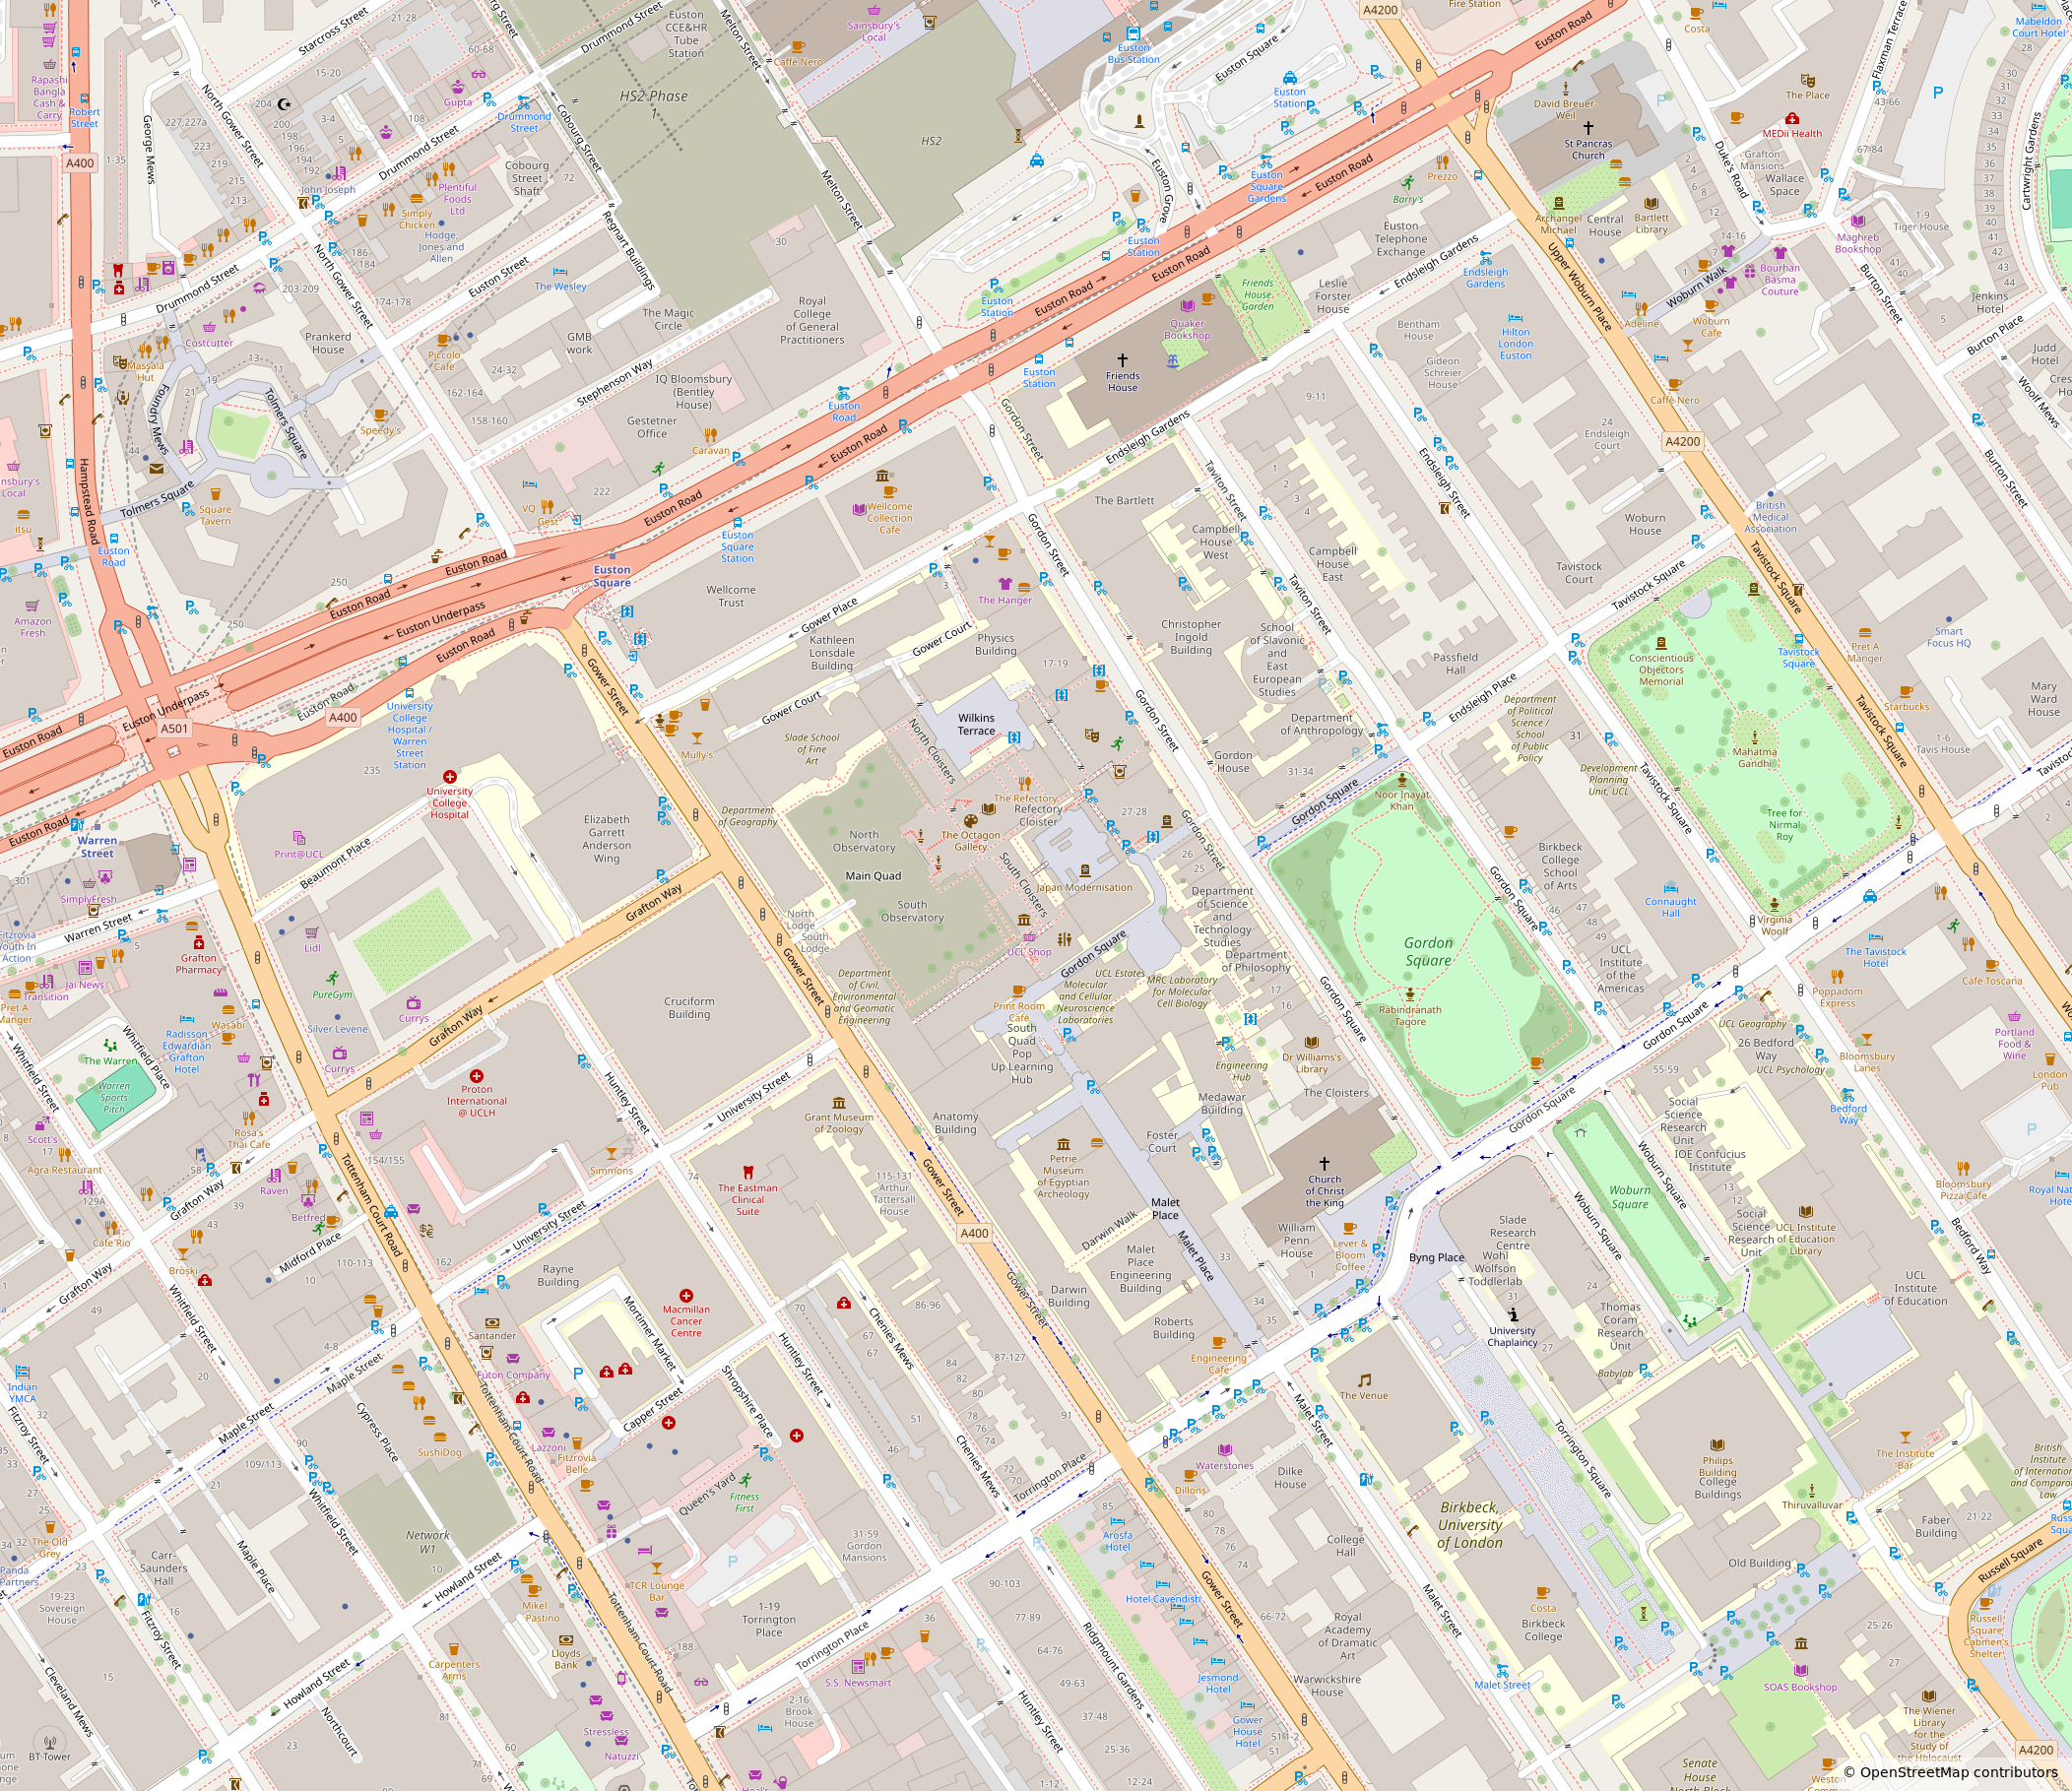
\includegraphics[width=0.70\textwidth]{images/ucl_bloomsbury_campus.png}
    \caption{Map of UCL's Bloomsbury Campus extracted from OpenStreetMap data.}
\end{figure}

Although the data from OpenStreetMap provides a lot of useful information, we will supplement it with Google Street View -- featured in the Google Maps software -- to find out more precise information such as lane markings and widths. Street View provides interactive panoramas from positions along the streets.

\section{Simulation of Urban MObility}
Simulation of Urban MObility (SUMO) is an open source, multi-modal traffic simulation package designed to handle large networks. It allows for intermodal simulation including pedestrians and comes with a large set of tools for scenario creation.

\section{Summary}
The main chapters should have a short summary, highlighting what the chapter has covered and any key points that need emphasising.

\chapter{Title of third chapter}
If you have a formal theorem you might try this.
\begin{definition}\label{def}
See definition~\ref{def}.
\end{definition}
\begin{theorem}
For all $n\in\nats,\; 1^n=1$.
\end{theorem}
\begin{proof}
By induction over $n$.
\end{proof}

\chapter{etc.}


\chapter{Conclusions}
\section{Achievements}
Summarise the achievements to confirm the project goals have been met.
\section{Evaluation}
Evaluation of the work (this may be in a separate chapter if there is substantial evaluation).

\section{Future Work}
How the project might be continued, but don't give the impression you ran out of time!

\appendix


\begin{thebibliography}{HHM99}


\bibitem[Pri70]{PriorNOP70}  %%only an example
A.~Prior.
\newblock The notion of the present.
\newblock {\em Studium Generale}, 23:  245--248, 1970.


\bibitem[Rey97]{Rey:D}
M.~Reynolds.
\newblock A decidable temporal logic of parallelism.
\newblock {\em Notre Dame Journal of Formal Logic}, 38(3):  419--436,
  1997.

\bibitem[Tha17]{ThamesLeisureFacts2017}
Thames Leisure.
\newblock 12 amazing facts about London.
\newblock {\em Thames Leisure}, archived January 7, 2017.
\newblock Available at:
  https://web.archive.org/web/20170107005431/http://www.thamesleisure.co.uk/12-amazing-facts-london/.

\bibitem[FHW17]{FHWA_ASCT17}
Federal Highway Administration.
\newblock EDC-1: Adaptive Signal Control Technology.
\newblock {\em Federal Highway Administration}, 2017.
\newblock Available at:
  https://www.fhwa.dot.gov/innovation/everydaycounts/edc-1/asct.cfm.

\bibitem[HW08]{HaklayWeberOSM08}
M.~Haklay and P.~Weber.
\newblock OpenStreetMap: User-generated street maps.
\newblock {\em IEEE Pervasive Computing}, 7(4): 12--18, 2008.
\newblock doi:10.1109/MPRV.2008.80.

\end{thebibliography}

\chapter{Other appendices, e.g., code listing}
Put your appendix sections here

\end{document}